\documentclass[11pt]{article}
\usepackage[margin=1in]{geometry}
\usepackage{amsmath,amssymb,amsfonts,amsthm}
\usepackage{booktabs}
\usepackage{graphicx}
\usepackage{float}
\usepackage{xcolor}
\usepackage{hyperref}
\usepackage{algorithm}
\usepackage{algpseudocode}
\usepackage{tikz}
\usetikzlibrary{arrows.meta,positioning,decorations.pathreplacing}

\setlength{\parindent}{0pt}
\setlength{\parskip}{6pt}

\newcommand{\dd}{\mathrm{d}}
\newcommand{\pp}{\partial}
\newcommand{\bfn}{\mathbf{n}}
\newcommand{\bfJ}{\mathbf{J}}
\newcommand{\chat}{\hat{c}}
\newcommand{\phihat}{\hat{\phi}}
\newcommand{\etahat}{\hat{\eta}}
\newcommand{\Dhat}{\hat{D}}
\newcommand{\epshat}{\hat{\varepsilon}}
\newcommand{\khat}{\hat{k}}
\newcommand{\Rhat}{\hat{R}}
\newcommand{\Shat}{\hat{S}}
\newcommand{\ghat}{\hat{g}}
\newcommand{\ds}{\,\dd s}
\newcommand{\dx}{\,\dd x}

\theoremstyle{remark}
\newtheorem{remark}{Remark}

\title{Method of Manufactured Solutions for\\
  Poisson--Nernst--Planck Equations with\\
  Butler--Volmer Boundary Conditions}
\author{Jake Weinstein}
\date{\today}

\begin{document}
\maketitle

\begin{abstract}
  The Method of Manufactured Solutions (MMS) is a rigorous code verification
  technique that confirms a numerical implementation converges at the expected
  order of accuracy.
  %
  An existing MMS formulation for the Poisson--Nernst--Planck (PNP) system
  imposes Dirichlet boundary conditions on the entire boundary, which tests
  the volumetric PDE discretization but completely avoids exercising the
  Butler--Volmer (BV) flux boundary condition.
  %
  This document extends the MMS framework to include the nonlinear BV flux
  condition at the electrode boundary.
  %
  The key idea is that the manufactured solution's normal flux at the electrode
  generically does \emph{not} equal the BV rate evaluated at the manufactured
  concentrations and overpotential.
  %
  We derive a boundary correction source term that accounts for this mismatch,
  incorporate it into the weak formulation, and specify the complete modified
  problem that the code must solve.
  %
  Achieving the expected convergence rates on this modified problem
  simultaneously verifies the interior PDE discretization, the BV nonlinear
  flux implementation, and the coupling between them.
\end{abstract}

\tableofcontents
\newpage


%% ====================================================================
\section{Introduction: Why BV BCs Need Special Treatment in MMS}
\label{sec:intro}
%% ====================================================================

The Method of Manufactured Solutions (MMS) is a widely-used code verification
technique~\cite{roache2002,roy2004,salari2000}.
The procedure is:
\begin{enumerate}
  \item Choose smooth, non-polynomial ``manufactured'' solutions for all unknowns.
  \item Substitute them into the governing PDEs to compute volumetric source terms.
  \item Solve the \emph{modified} PDEs (with sources) numerically, using boundary
        and initial conditions evaluated from the manufactured solutions.
  \item Compare the numerical solution to the known exact solution; verify that
        the error decreases at the expected rate under mesh refinement.
\end{enumerate}

A standard MMS study for the PNP equations (as in the existing formulations
document) chooses manufactured solutions that vanish on $\pp\Omega$ and
imposes $c_i = c_i^{\mathrm{exact}}$, $\phi = \phi^{\mathrm{exact}}$ as
Dirichlet conditions everywhere.
This approach tests the volumetric discretization but \emph{completely bypasses}
the Butler--Volmer flux boundary condition---the most physically important and
numerically challenging part of the electrochemical problem.

To verify the BV implementation, we must choose manufactured solutions that
exercise the BV flux BC.
The essential observation is that, for a generic manufactured solution,
the diffusive/migratory flux at the electrode surface will \emph{not} equal
the BV reaction rate evaluated at the manufactured surface concentrations
and overpotential.
This mismatch requires an additional \emph{boundary source term} in the weak form.

This document derives the complete MMS framework, including:
\begin{itemize}
  \item The nondimensional PNP-BV strong form matching the \texttt{Forward/bv\_solver.py} implementation.
  \item Choice of manufactured solutions with justification.
  \item Volumetric source terms $\Shat_i$ and $\Shat_\phi$.
  \item Boundary source terms $\ghat_i$ for each species at the electrode.
  \item The complete modified weak formulation.
  \item Pseudocode for the implementation.
  \item Expected convergence rates.
\end{itemize}


%% ====================================================================
\section{The PNP--BV System (Nondimensional)}
\label{sec:system}
%% ====================================================================

We work entirely in nondimensional variables (hatted quantities), matching the
solver conventions.
The reference scales are: $L$ (length), $D_{\mathrm{ref}}$ (diffusivity),
$c_{\mathrm{ref}}$ (concentration), $V_T = RT/F$ (thermal voltage),
$\tau = L^2/D_{\mathrm{ref}}$ (time), $\kappa = D_{\mathrm{ref}}/L$
(velocity / rate constant).

\subsection{Domain and boundaries}

The domain is the unit square $\Omega = [0,1]^2$ with boundary decomposition
(see Figure~\ref{fig:domain}):
\begin{align}
  \Gamma_{\mathrm{elec}} &= \{(x,0) : x\in[0,1]\}
  &&\text{(bottom, $y=0$: electrode)}, \label{eq:Gelec}\\
  \Gamma_{\mathrm{bulk}} &= \{(x,1) : x\in[0,1]\}
  &&\text{(top, $y=1$: bulk)}, \\
  \Gamma_{\mathrm{side}} &= \{(0,y),(1,y) : y\in[0,1]\}
  &&\text{(left/right: insulating walls)}.
\end{align}

\begin{figure}[h]
\centering
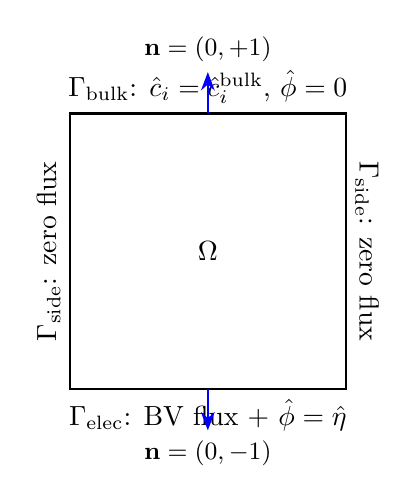
\begin{tikzpicture}[scale=3.5]
  % Domain
  \draw[thick] (0,0) rectangle (1,1);
  % Labels
  \node[below] at (0.5,0) {$\Gamma_{\mathrm{elec}}$: BV flux + $\phihat = \etahat$};
  \node[above] at (0.5,1) {$\Gamma_{\mathrm{bulk}}$: $\chat_i = \chat_i^{\mathrm{bulk}}$, $\phihat = 0$};
  \node[left,rotate=90,anchor=south] at (0,0.5) {$\Gamma_{\mathrm{side}}$: zero flux};
  \node[right,rotate=-90,anchor=south] at (1,0.5) {$\Gamma_{\mathrm{side}}$: zero flux};
  % Interior label
  \node at (0.5,0.5) {$\Omega$};
  % Normal vectors
  \draw[-{Stealth},thick,blue] (0.5,0) -- (0.5,-0.15) node[below,black]
    {\small $\bfn = (0,-1)$};
  \draw[-{Stealth},thick,blue] (0.5,1) -- (0.5,1.15) node[above,black]
    {\small $\bfn = (0,+1)$};
\end{tikzpicture}
\caption{Domain $\Omega = [0,1]^2$ and boundary segments.  The outward unit
  normal on the electrode $\Gamma_{\mathrm{elec}}$ is $\bfn = (0,-1)$.}
\label{fig:domain}
\end{figure}


\subsection{Governing equations}

\paragraph{Nernst--Planck equation} for species $i = 1,\ldots,n$:
\begin{equation}\label{eq:NP}
  \frac{\pp \chat_i}{\pp \hat{t}}
  = \nabla \cdot \bigl[\Dhat_i (\nabla \chat_i + z_i \chat_i \nabla \phihat)\bigr]
  \quad \text{in } \Omega.
\end{equation}
Here $z_i$ is the valence, $\Dhat_i$ the nondimensional diffusivity, and the
electromigration prefactor (which is unity after nondimensionalization with
$V_T$) has been absorbed.

\paragraph{Poisson equation:}
\begin{equation}\label{eq:Poisson}
  -\epshat\, \nabla^2 \phihat = \sum_{i=1}^{n} z_i \chat_i
  \quad \text{in } \Omega,
\end{equation}
where $\epshat = (\lambda_D / L)^2$ is the squared Debye-length ratio.

\subsection{Boundary conditions}

\paragraph{Electrode ($\Gamma_{\mathrm{elec}}$, $y=0$):}
\begin{itemize}
  \item \textbf{Species:} Butler--Volmer flux condition.
    For each reaction $j$ with stoichiometric coefficients $s_{ij}$:
    \begin{equation}\label{eq:BV_flux_BC}
      -\Dhat_i \bigl(\nabla \chat_i + z_i \chat_i \nabla \phihat\bigr) \cdot \bfn
      \;=\; \sum_j s_{ij}\, \Rhat_j,
    \end{equation}
    where $\bfn = (0,-1)$ is the outward normal (pointing into the electrode).
  \item \textbf{Potential:} Dirichlet, $\phihat = \etahat$ (applied overpotential
    in thermal voltage units).
\end{itemize}

\paragraph{Bulk ($\Gamma_{\mathrm{bulk}}$, $y=1$):}
\begin{itemize}
  \item $\chat_i = \chat_i^{\mathrm{bulk}}$ (Dirichlet).
  \item $\phihat = 0$ (ground).
\end{itemize}

\paragraph{Sides ($\Gamma_{\mathrm{side}}$):}
\begin{itemize}
  \item Zero-flux (homogeneous Neumann) for all species and potential.
\end{itemize}


\subsection{Butler--Volmer reaction rates}
\label{sec:BV_rates}

For the O$_2$ reduction system, two reactions couple the species
O$_2$ ($i=0$) and H$_2$O$_2$ ($i=1$):
\begin{align}
  \Rhat_1 &= \khat_{0,1}\Bigl[
    \chat_{\mathrm{O}_2}\, \exp(-\alpha_1 \etahat)
    - \chat_{\mathrm{ref},1}\, \exp\bigl((1-\alpha_1)\etahat\bigr)
  \Bigr],
  \label{eq:R1}\\[4pt]
  \Rhat_2 &= \khat_{0,2}\, \chat_{\mathrm{H}_2\mathrm{O}_2}\,
    \exp(-\alpha_2 \etahat),
  \label{eq:R2}
\end{align}
with stoichiometry matrix:
\begin{equation}\label{eq:stoichiometry}
  \mathbf{s} =
  \begin{pmatrix}
    s_{0,1} & s_{0,2} \\
    s_{1,1} & s_{1,2}
  \end{pmatrix}
  =
  \begin{pmatrix}
    -1 & \phantom{-}0 \\
    +1 & -1
  \end{pmatrix}.
\end{equation}
Species 0 (O$_2$) is consumed by $\Rhat_1$; species 1 (H$_2$O$_2$)
is produced by $\Rhat_1$ and consumed by $\Rhat_2$.

\begin{remark}[General multi-reaction form]
For a general system with $n$ species and $m$ reactions, the BV flux BC
for species $i$ at the electrode is:
\begin{equation}\label{eq:BV_general}
  -\Dhat_i(\nabla \chat_i + z_i \chat_i \nabla\phihat)\cdot\bfn
  = \sum_{j=1}^{m} s_{ij}\, \Rhat_j.
\end{equation}
The MMS framework presented below holds for any number of species and reactions.
\end{remark}

\begin{remark}[Sign convention in the solver]
In the solver (\texttt{bv\_solver.py}), the BV flux enters the weak form as
\[
  F_{\mathrm{res}} \mathrel{-}= s_{ij}\, \Rhat_j\, v_i\, \dd s(\text{electrode}),
\]
which arises from integration by parts:  the boundary integral from IBP is
$+\int_{\Gamma} \Dhat_i(\nabla\chat_i + z_i \chat_i \nabla\phihat)\cdot\bfn\, v_i \ds$,
and substituting the BV condition \eqref{eq:BV_flux_BC} gives
$-\sum_j s_{ij} \Rhat_j\, v_i$ on the electrode.
\end{remark}


%% ====================================================================
\section{Weak Formulation (No MMS Sources)}
\label{sec:weak}
%% ====================================================================

Before introducing manufactured solutions, we state the weak form that the solver
implements.
Let $v_i, w \in H^1(\Omega)$ be test functions with $v_i = 0$ on $\Gamma_{\mathrm{bulk}}$
(where Dirichlet BCs are imposed on $\chat_i$) and $w = 0$ on $\Gamma_{\mathrm{elec}}
\cup \Gamma_{\mathrm{bulk}}$ (Dirichlet BCs on $\phihat$).

\paragraph{Nernst--Planck:}
\begin{multline}\label{eq:NP_weak}
  \int_\Omega \frac{\pp\chat_i}{\pp\hat{t}}\, v_i \dx
  + \int_\Omega \Dhat_i\bigl(\nabla\chat_i + z_i \chat_i \nabla\phihat\bigr)
    \cdot \nabla v_i \dx \\
  = -\sum_{j} \int_{\Gamma_{\mathrm{elec}}} s_{ij}\, \Rhat_j\, v_i \ds
  \quad \forall\, v_i.
\end{multline}
The sign on the right-hand side is negative because the boundary integral
from IBP gives
$+\int_{\Gamma} \bfJ_i \cdot \bfn\, v_i \ds$,
and $\bfJ_i \cdot \bfn = -\sum_j s_{ij} \Rhat_j$ from the BV condition.
Hence the boundary term is $-\sum_j s_{ij} \Rhat_j \, v_i$.

On $\Gamma_{\mathrm{side}}$, the zero-flux condition makes the boundary
integral vanish.
On $\Gamma_{\mathrm{bulk}}$, $v_i = 0$ by the Dirichlet lift.

\paragraph{Poisson:}
\begin{equation}\label{eq:Poisson_weak}
  \int_\Omega \epshat\, \nabla\phihat \cdot \nabla w \dx
  = \int_\Omega \biggl(\sum_{i=1}^{n} z_i \chat_i\biggr) w \dx
  \quad \forall\, w.
\end{equation}
(The Neumann integral on $\Gamma_{\mathrm{side}}$ vanishes by the zero-flux
condition, and $w = 0$ on the Dirichlet boundaries.)


%% ====================================================================
\section{Choice of Manufactured Solutions}
\label{sec:manufactured}
%% ====================================================================

\subsection{Design requirements}

The manufactured solutions must satisfy:
\begin{enumerate}
  \item \textbf{Positivity:} $\chat_i^{\mathrm{ex}}(x,y) > 0$ everywhere (physical concentrations).
  \item \textbf{Non-polynomial:} Cannot be exactly represented by the finite element basis,
    so that the discretization error is nonzero.
  \item \textbf{Smoothness:} $C^\infty$ to avoid polluting the convergence study with regularity issues.
  \item \textbf{Nonzero normal flux at $y=0$:}
    The manufactured flux at the electrode should be nonzero, to exercise the BV BC.
  \item \textbf{Zero normal flux at $x=0,1$:}
    To be compatible with the zero-flux side walls (or else we would need side-wall
    correction sources too).
  \item \textbf{Compatibility with Dirichlet BCs at $y=1$:}
    The values $\chat_i^{\mathrm{ex}}(x,1)$ and $\phihat^{\mathrm{ex}}(x,1)$
    define the Dirichlet data on the bulk boundary.
\end{enumerate}

\subsection{Proposed manufactured solutions}

We propose the following steady-state manufactured solutions (dropping the
hat notation for brevity within this section; all quantities are nondimensional):

\begin{equation}\label{eq:ci_exact}
  \boxed{
    c_i^{\mathrm{ex}}(x,y) = c_{0,i} + A_i \cos(\pi x)\,
    \bigl(1 - e^{-\beta_i y}\bigr)
  }
\end{equation}

\begin{equation}\label{eq:phi_exact}
  \boxed{
    \phi^{\mathrm{ex}}(x,y) = \eta_0\, (1-y) + B\, \cos(\pi x)\, y\,(1-y)
  }
\end{equation}

\paragraph{Parameters:}
\begin{itemize}
  \item $c_{0,i} > 0$: background (bulk) concentration for species $i$
    (e.g., $c_{0,0} = c_{0,1} = 1.0$).
  \item $A_i$: amplitude of the concentration perturbation (e.g., $A_i = 0.2$).
    Choose $|A_i| < c_{0,i}$ to ensure positivity.
  \item $\beta_i > 0$: controls the boundary-layer steepness
    (e.g., $\beta_i = 3$).
  \item $\eta_0$: the nominal electrode overpotential (matching the
    solver's $\etahat$).
  \item $B$: amplitude of the potential perturbation (e.g., $B = 0.1$).
\end{itemize}

\subsection{Verification of design requirements}

\paragraph{Positivity.}
At any $(x,y)$:
\[
  c_i^{\mathrm{ex}} \geq c_{0,i} - |A_i|\, |1 - e^{-\beta_i y}|
  \geq c_{0,i} - |A_i| > 0
\]
provided $|A_i| < c_{0,i}$.

\paragraph{Non-polynomial.}
The $\cos(\pi x)$ and $e^{-\beta_i y}$ factors are transcendental.

\paragraph{Smoothness.}
Both expressions are $C^\infty(\bar{\Omega})$.

\paragraph{Nonzero flux at $y=0$ (electrode).}
We compute:
\[
  \frac{\pp c_i^{\mathrm{ex}}}{\pp y}\bigg|_{y=0}
  = A_i\, \beta_i\, \cos(\pi x)\, e^{-\beta_i \cdot 0}
  = A_i\, \beta_i\, \cos(\pi x)
  \neq 0.
\]
This is the key property: the manufactured solution has a nonzero diffusive
flux at the electrode, which generically differs from the BV rate
$\sum_j s_{ij} \Rhat_j$.

\paragraph{Zero $x$-flux at $x=0,1$.}
\[
  \frac{\pp c_i^{\mathrm{ex}}}{\pp x} = -A_i\, \pi\, \sin(\pi x)\,
  (1 - e^{-\beta_i y}),
\]
which vanishes at $x = 0$ and $x = 1$ since $\sin(0) = \sin(\pi) = 0$.
Similarly,
\[
  \frac{\pp \phi^{\mathrm{ex}}}{\pp x} = -B\, \pi\, \sin(\pi x)\, y(1-y),
\]
which also vanishes at $x = 0, 1$.
Thus the zero-flux condition on $\Gamma_{\mathrm{side}}$ is automatically
satisfied by both $c_i^{\mathrm{ex}}$ and $\phi^{\mathrm{ex}}$,
and \textbf{no side-wall correction source is needed}.

\paragraph{Dirichlet values.}
At $y = 1$ (bulk):
\[
  c_i^{\mathrm{ex}}(x,1) = c_{0,i} + A_i \cos(\pi x)\,(1 - e^{-\beta_i}),
\]
which is the Dirichlet BC value for $\chat_i$ on $\Gamma_{\mathrm{bulk}}$.
\[
  \phi^{\mathrm{ex}}(x,1) = 0,
\]
which matches the ground condition $\phihat = 0$.

At $y = 0$ (electrode):
\[
  c_i^{\mathrm{ex}}(x,0) = c_{0,i}
  \qquad\text{(uniform, $x$-independent)},
\]
\[
  \phi^{\mathrm{ex}}(x,0) = \eta_0,
\]
which matches the electrode Dirichlet condition $\phihat = \etahat$ if we set
$\etahat = \eta_0$.


%% ====================================================================
\section{Volume Source Terms}
\label{sec:volume_sources}
%% ====================================================================

Substituting the manufactured solutions into the PDEs yields residuals that
become the volumetric forcing functions.
We work in steady state ($\pp \chat_i / \pp \hat{t} = 0$) for simplicity;
the time-dependent extension is straightforward.

\subsection{Derivatives of the manufactured concentration}

Let $f_i(y) = 1 - e^{-\beta_i y}$ so that
$c_i^{\mathrm{ex}} = c_{0,i} + A_i \cos(\pi x)\, f_i(y)$.

First-order derivatives:
\begin{align}
  \frac{\pp c_i^{\mathrm{ex}}}{\pp x}
  &= -A_i\, \pi\, \sin(\pi x)\, f_i(y),
  \label{eq:dcx}\\
  \frac{\pp c_i^{\mathrm{ex}}}{\pp y}
  &= A_i\, \beta_i\, \cos(\pi x)\, e^{-\beta_i y}.
  \label{eq:dcy}
\end{align}

Second-order derivatives:
\begin{align}
  \frac{\pp^2 c_i^{\mathrm{ex}}}{\pp x^2}
  &= -A_i\, \pi^2\, \cos(\pi x)\, f_i(y),
  \label{eq:d2cx}\\
  \frac{\pp^2 c_i^{\mathrm{ex}}}{\pp y^2}
  &= -A_i\, \beta_i^2\, \cos(\pi x)\, e^{-\beta_i y}.
  \label{eq:d2cy}
\end{align}

Laplacian:
\begin{equation}\label{eq:lapc}
  \nabla^2 c_i^{\mathrm{ex}}
  = -A_i \cos(\pi x)\bigl[\pi^2 f_i(y) + \beta_i^2 e^{-\beta_i y}\bigr].
\end{equation}

\subsection{Derivatives of the manufactured potential}

Let $\phi^{\mathrm{ex}} = \eta_0(1-y) + B \cos(\pi x)\, y(1-y)$.

First-order derivatives:
\begin{align}
  \frac{\pp \phi^{\mathrm{ex}}}{\pp x}
  &= -B\, \pi\, \sin(\pi x)\, y(1-y),
  \label{eq:dphix}\\
  \frac{\pp \phi^{\mathrm{ex}}}{\pp y}
  &= -\eta_0 + B\, \cos(\pi x)\,(1-2y).
  \label{eq:dphiy}
\end{align}

Second-order derivatives:
\begin{align}
  \frac{\pp^2 \phi^{\mathrm{ex}}}{\pp x^2}
  &= -B\, \pi^2\, \cos(\pi x)\, y(1-y),
  \label{eq:d2phix}\\
  \frac{\pp^2 \phi^{\mathrm{ex}}}{\pp y^2}
  &= -2B\, \cos(\pi x).
  \label{eq:d2phiy}
\end{align}

Laplacian:
\begin{equation}\label{eq:lapphi}
  \nabla^2 \phi^{\mathrm{ex}}
  = -B\cos(\pi x)\bigl[\pi^2 y(1-y) + 2\bigr].
\end{equation}


\subsection{Species source term $\Shat_i$}

The strong-form residual of the Nernst--Planck equation at the manufactured
solution is:
\begin{equation}\label{eq:Si_def}
  \Shat_i
  = \underbrace{\frac{\pp c_i^{\mathrm{ex}}}{\pp\hat{t}}}_{= 0 \text{ (steady state)}}
  - \nabla\cdot\Bigl[\Dhat_i\bigl(\nabla c_i^{\mathrm{ex}}
    + z_i c_i^{\mathrm{ex}} \nabla\phi^{\mathrm{ex}}\bigr)\Bigr].
\end{equation}

Expanding the divergence:
\begin{equation}\label{eq:div_flux}
  \nabla\cdot\bigl[\Dhat_i(\nabla c_i^{\mathrm{ex}} + z_i c_i^{\mathrm{ex}}
  \nabla\phi^{\mathrm{ex}})\bigr]
  = \Dhat_i\Bigl[
    \nabla^2 c_i^{\mathrm{ex}}
    + z_i\bigl(\nabla c_i^{\mathrm{ex}} \cdot \nabla\phi^{\mathrm{ex}}
      + c_i^{\mathrm{ex}}\, \nabla^2\phi^{\mathrm{ex}}\bigr)
  \Bigr].
\end{equation}

The gradient inner product is:
\begin{equation}\label{eq:grad_dot}
  \nabla c_i^{\mathrm{ex}} \cdot \nabla\phi^{\mathrm{ex}}
  = \frac{\pp c_i^{\mathrm{ex}}}{\pp x}\,\frac{\pp\phi^{\mathrm{ex}}}{\pp x}
  + \frac{\pp c_i^{\mathrm{ex}}}{\pp y}\,\frac{\pp\phi^{\mathrm{ex}}}{\pp y}.
\end{equation}

Using \eqref{eq:dcx}--\eqref{eq:dphiy}:
\begin{align}
  \frac{\pp c_i^{\mathrm{ex}}}{\pp x}\,\frac{\pp\phi^{\mathrm{ex}}}{\pp x}
  &= A_i B\, \pi^2\, \sin^2(\pi x)\, f_i(y)\, y(1-y),
  \label{eq:cross_xx}\\[4pt]
  \frac{\pp c_i^{\mathrm{ex}}}{\pp y}\,\frac{\pp\phi^{\mathrm{ex}}}{\pp y}
  &= A_i\, \beta_i\, \cos(\pi x)\, e^{-\beta_i y}\,
    \bigl[-\eta_0 + B\cos(\pi x)(1-2y)\bigr].
  \label{eq:cross_yy}
\end{align}

Therefore:
\begin{equation}\label{eq:Si_final}
  \boxed{
  \Shat_i = -\Dhat_i\Bigl[
    \nabla^2 c_i^{\mathrm{ex}}
    + z_i\bigl(
      \nabla c_i^{\mathrm{ex}} \cdot \nabla\phi^{\mathrm{ex}}
      + c_i^{\mathrm{ex}}\, \nabla^2\phi^{\mathrm{ex}}
    \bigr)
  \Bigr]
  }
\end{equation}
where each term is given by the expressions above.

\begin{remark}[Implementation]
In practice, $\Shat_i$ is evaluated symbolically using SymPy (or by direct
UFL differentiation in Firedrake) rather than by hand-coding
\eqref{eq:cross_xx}--\eqref{eq:cross_yy}.
The analytic expressions above serve as a cross-check.
\end{remark}

\subsection{Poisson source term $\Shat_\phi$}

From the Poisson equation \eqref{eq:Poisson}:
\begin{equation}\label{eq:Sphi_def}
  \Shat_\phi
  = -\epshat\, \nabla^2\phi^{\mathrm{ex}} - \sum_{i=1}^{n} z_i\, c_i^{\mathrm{ex}}.
\end{equation}

Using \eqref{eq:lapphi}:
\begin{equation}\label{eq:Sphi_final}
  \boxed{
  \Shat_\phi = \epshat\, B\cos(\pi x)\bigl[\pi^2 y(1-y) + 2\bigr]
  - \sum_{i=1}^{n} z_i\, c_i^{\mathrm{ex}}(x,y)
  }
\end{equation}

For a charge-neutral system (e.g., $z_0 = z_1 = 0$ for neutral O$_2$/H$_2$O$_2$),
the summation vanishes and $\Shat_\phi$ depends only on $\phi^{\mathrm{ex}}$.


%% ====================================================================
\section{Boundary Source Terms for Butler--Volmer BCs}
\label{sec:bv_source}
%% ====================================================================

This is the central new contribution.
On the electrode $\Gamma_{\mathrm{elec}}$ ($y = 0$), the physical BV
boundary condition states:
\begin{equation}\label{eq:BV_phys}
  \underbrace{-\Dhat_i(\nabla\chat_i + z_i \chat_i \nabla\phihat)\cdot\bfn}_{%
    \text{total flux leaving domain}}
  = \sum_j s_{ij}\, \Rhat_j(\chat|_{\mathrm{surf}}, \etahat).
\end{equation}

When $\chat_i = c_i^{\mathrm{ex}}$ and $\phihat = \phi^{\mathrm{ex}}$, the
left-hand side is the \emph{manufactured flux}:
\begin{equation}\label{eq:Fmanuf}
  \mathcal{F}_i^{\mathrm{ex}}(x)
  \;=\; -\Dhat_i\bigl(\nabla c_i^{\mathrm{ex}} + z_i c_i^{\mathrm{ex}}
  \nabla\phi^{\mathrm{ex}}\bigr)\cdot\bfn\bigg|_{y=0},
\end{equation}
and the right-hand side is the \emph{manufactured BV rate}:
\begin{equation}\label{eq:BVmanuf}
  \mathcal{B}_i^{\mathrm{ex}}(x)
  \;=\; \sum_j s_{ij}\, \Rhat_j\bigl(c^{\mathrm{ex}}(x,0),\, \phi^{\mathrm{ex}}(x,0)\bigr).
\end{equation}

In general, $\mathcal{F}_i^{\mathrm{ex}} \neq \mathcal{B}_i^{\mathrm{ex}}$,
so we define the \textbf{boundary source term}:
\begin{equation}\label{eq:gi_def}
  \boxed{
    \ghat_i(x) = \mathcal{F}_i^{\mathrm{ex}}(x) - \mathcal{B}_i^{\mathrm{ex}}(x)
  }
\end{equation}

This is the mismatch between the flux that the manufactured solution actually
has and the flux that the BV kinetics would demand.
Adding $\ghat_i$ as an extra boundary source ``absorbs'' this mismatch, ensuring
that $c_i^{\mathrm{ex}}$ and $\phi^{\mathrm{ex}}$ satisfy the modified problem
exactly.


\subsection{Explicit computation of $\mathcal{F}_i^{\mathrm{ex}}$}

On $\Gamma_{\mathrm{elec}}$, $\bfn = (0, -1)$, so:
\begin{equation}
  \mathcal{F}_i^{\mathrm{ex}}(x)
  = \Dhat_i \biggl(
    \frac{\pp c_i^{\mathrm{ex}}}{\pp y}
    + z_i\, c_i^{\mathrm{ex}}\, \frac{\pp\phi^{\mathrm{ex}}}{\pp y}
  \biggr)\bigg|_{y=0}.
\end{equation}
(The sign flip from $\bfn = (0,-1)$ cancels with the minus in \eqref{eq:Fmanuf}.)

Evaluating at $y=0$:
\begin{align}
  \frac{\pp c_i^{\mathrm{ex}}}{\pp y}\bigg|_{y=0}
  &= A_i\, \beta_i\, \cos(\pi x),
  \label{eq:dcy0}\\
  c_i^{\mathrm{ex}}(x,0) &= c_{0,i},
  \label{eq:c0}\\
  \frac{\pp\phi^{\mathrm{ex}}}{\pp y}\bigg|_{y=0}
  &= -\eta_0 + B\, \cos(\pi x).
  \label{eq:dphiy0}
\end{align}

Therefore:
\begin{equation}\label{eq:Fi_explicit}
  \boxed{
  \mathcal{F}_i^{\mathrm{ex}}(x)
  = \Dhat_i\bigl[
    A_i\, \beta_i\, \cos(\pi x)
    + z_i\, c_{0,i}\, \bigl(-\eta_0 + B\cos(\pi x)\bigr)
  \bigr]
  }
\end{equation}

\paragraph{Neutral species ($z_i = 0$):}
\[
  \mathcal{F}_i^{\mathrm{ex}}(x) = \Dhat_i\, A_i\, \beta_i\, \cos(\pi x)
  \qquad (z_i = 0).
\]
This is purely diffusive and varies with $x$.


\subsection{Explicit computation of $\mathcal{B}_i^{\mathrm{ex}}$}

The BV rates are evaluated at the manufactured surface values.
From Section~\ref{sec:BV_rates}:
\begin{align}
  \Rhat_1^{\mathrm{ex}}
  &= \khat_{0,1}\bigl[
    c_{0,0}\, e^{-\alpha_1 \eta_0}
    - \chat_{\mathrm{ref},1}\, e^{(1-\alpha_1)\eta_0}
  \bigr],
  \label{eq:R1ex}\\
  \Rhat_2^{\mathrm{ex}}
  &= \khat_{0,2}\, c_{0,1}\, e^{-\alpha_2 \eta_0}.
  \label{eq:R2ex}
\end{align}
Note that these are \emph{constants} (independent of $x$) because
$c_i^{\mathrm{ex}}(x,0) = c_{0,i}$ and $\phi^{\mathrm{ex}}(x,0) = \eta_0$
are both $x$-independent.

For the two-species, two-reaction system:
\begin{align}
  \mathcal{B}_0^{\mathrm{ex}}
  &= s_{0,1}\,\Rhat_1^{\mathrm{ex}} + s_{0,2}\,\Rhat_2^{\mathrm{ex}}
  = -\Rhat_1^{\mathrm{ex}},
  \label{eq:B0ex}\\
  \mathcal{B}_1^{\mathrm{ex}}
  &= s_{1,1}\,\Rhat_1^{\mathrm{ex}} + s_{1,2}\,\Rhat_2^{\mathrm{ex}}
  = \Rhat_1^{\mathrm{ex}} - \Rhat_2^{\mathrm{ex}}.
  \label{eq:B1ex}
\end{align}


\subsection{Final boundary source terms}

Combining \eqref{eq:Fi_explicit} and \eqref{eq:B0ex}--\eqref{eq:B1ex}:

\begin{equation}\label{eq:g0}
  \ghat_0(x) = \Dhat_0\, A_0\, \beta_0\, \cos(\pi x)
  + z_0\, \Dhat_0\, c_{0,0}\,(-\eta_0 + B\cos(\pi x))
  + \Rhat_1^{\mathrm{ex}},
\end{equation}

\begin{equation}\label{eq:g1}
  \ghat_1(x) = \Dhat_1\, A_1\, \beta_1\, \cos(\pi x)
  + z_1\, \Dhat_1\, c_{0,1}\,(-\eta_0 + B\cos(\pi x))
  - \Rhat_1^{\mathrm{ex}} + \Rhat_2^{\mathrm{ex}}.
\end{equation}

\begin{remark}[Neutral species simplification]
For neutral species ($z_0 = z_1 = 0$), the electromigration terms vanish:
\begin{align}
  \ghat_0(x) &= \Dhat_0\, A_0\, \beta_0\, \cos(\pi x) + \Rhat_1^{\mathrm{ex}},\\
  \ghat_1(x) &= \Dhat_1\, A_1\, \beta_1\, \cos(\pi x)
  - \Rhat_1^{\mathrm{ex}} + \Rhat_2^{\mathrm{ex}}.
\end{align}
Note that $\ghat_i$ has both a spatially-varying part (from the manufactured flux)
and a constant part (from the BV rates).
\end{remark}


%% ====================================================================
\section{Complete Modified Weak Formulation}
\label{sec:modified_weak}
%% ====================================================================

The MMS problem is: find $(\chat_i, \phihat) \in V_h$ such that

\paragraph{Nernst--Planck (steady state):}
\begin{multline}\label{eq:NP_MMS}
  \int_\Omega \Dhat_i\bigl(\nabla\chat_i + z_i \chat_i \nabla\phihat\bigr)
    \cdot \nabla v_i \dx
  = \int_\Omega \Shat_i\, v_i \dx \\
  -\sum_j \int_{\Gamma_{\mathrm{elec}}} s_{ij}\, \Rhat_j(\chat|_{\mathrm{surf}},
    \phihat|_{\mathrm{surf}})\, v_i \ds
  - \int_{\Gamma_{\mathrm{elec}}} \ghat_i\, v_i \ds
  \quad \forall\, v_i \in V_h^0,
\end{multline}
where $V_h^0$ denotes the test space with functions vanishing on
$\Gamma_{\mathrm{bulk}}$ (the Dirichlet boundary for $\chat_i$).

\paragraph{Poisson:}
\begin{equation}\label{eq:Poisson_MMS}
  \int_\Omega \epshat\, \nabla\phihat \cdot \nabla w \dx
  = \int_\Omega \biggl(\sum_{i=1}^{n} z_i\, \chat_i\biggr) w \dx
  + \int_\Omega \Shat_\phi\, w \dx
  \quad \forall\, w \in W_h^0.
\end{equation}

\paragraph{Boundary conditions:}
\begin{alignat}{3}
  &\chat_i = c_i^{\mathrm{ex}}(x,1) &\quad &\text{on } \Gamma_{\mathrm{bulk}},
  \label{eq:MMS_bc_c_bulk}\\
  &\phihat = 0 &\quad &\text{on } \Gamma_{\mathrm{bulk}},
  \label{eq:MMS_bc_phi_bulk}\\
  &\phihat = \eta_0 &\quad &\text{on } \Gamma_{\mathrm{elec}},
  \label{eq:MMS_bc_phi_elec}\\
  &\text{BV flux + source } \ghat_i &\quad &\text{on } \Gamma_{\mathrm{elec}}
    \text{ (natural BC, in weak form)},
  \label{eq:MMS_bc_c_elec}\\
  &\text{zero flux} &\quad &\text{on } \Gamma_{\mathrm{side}}.
  \label{eq:MMS_bc_side}
\end{alignat}

\subsection{Interpretation of each term}

Equation~\eqref{eq:NP_MMS} has three right-hand side contributions:
\begin{enumerate}
  \item \textbf{Volume source} $\Shat_i$:
    Compensates for the fact that $c_i^{\mathrm{ex}}$ does not satisfy the PDE
    $\nabla \cdot \bfJ_i = 0$ in the interior.
  \item \textbf{BV flux} $\Rhat_j$:
    The actual Butler--Volmer reaction rate, computed from the \emph{numerical}
    solution's surface concentrations and the overpotential $\etahat$.
    This is the term that exercises the BV boundary condition implementation.
  \item \textbf{Boundary correction source} $\ghat_i$:
    A \emph{known, precomputed} function of $x$ (since it depends only on
    the manufactured solution).
    It corrects for the mismatch between the manufactured flux and the BV rate.
    Crucially, $\ghat_i$ is \emph{not} a function of the numerical unknowns ---
    it is data, like $\Shat_i$.
\end{enumerate}

\subsection{Why this works}

When $(\chat_i, \phihat) = (c_i^{\mathrm{ex}}, \phi^{\mathrm{ex}})$, each term
in \eqref{eq:NP_MMS} satisfies:
\begin{itemize}
  \item LHS $ = \int_\Omega \Dhat_i(\nabla c_i^{\mathrm{ex}} + z_i c_i^{\mathrm{ex}}
    \nabla\phi^{\mathrm{ex}}) \cdot \nabla v_i \dx$.

  \item RHS term 1: $\int_\Omega \Shat_i\, v_i \dx$, where
    $\Shat_i = -\nabla\cdot[\Dhat_i(\nabla c_i^{\mathrm{ex}} + z_i c_i^{\mathrm{ex}}
    \nabla\phi^{\mathrm{ex}})]$.

  \item RHS terms 2+3:
    $-\sum_j s_{ij} \Rhat_j^{\mathrm{ex}} v_i - \ghat_i v_i
    = -\mathcal{B}_i^{\mathrm{ex}} v_i - (\mathcal{F}_i^{\mathrm{ex}}
    - \mathcal{B}_i^{\mathrm{ex}}) v_i
    = -\mathcal{F}_i^{\mathrm{ex}} v_i$.
\end{itemize}

Integrating by parts on the LHS:
\begin{align}
  \text{LHS} &= -\int_\Omega \nabla\cdot[\Dhat_i(\cdots)]\, v_i \dx
    + \int_{\Gamma_{\mathrm{elec}}} \Dhat_i(\cdots)\cdot\bfn\, v_i \ds
    \notag\\
  &= \int_\Omega \Shat_i\, v_i \dx - \int_{\Gamma_{\mathrm{elec}}}
    \mathcal{F}_i^{\mathrm{ex}}\, v_i \ds.
\end{align}
This equals the RHS, confirming that $c_i^{\mathrm{ex}}$ is an exact solution
of the modified problem.

\subsection{Residual form for the solver}

In the solver's residual-form convention ($F_{\mathrm{res}} = 0$ at the
solution), the MMS weak form is:

\begin{multline}\label{eq:Fres_MMS}
  F_{\mathrm{res}} = \sum_{i=1}^{n} \biggl[
    \int_\Omega \Dhat_i(\nabla\chat_i + z_i \chat_i \nabla\phihat)\cdot\nabla v_i \dx
    - \int_\Omega \Shat_i\, v_i \dx \\
    + \sum_j s_{ij}\int_{\Gamma_{\mathrm{elec}}} \Rhat_j\, v_i \ds
    + \int_{\Gamma_{\mathrm{elec}}} \ghat_i\, v_i \ds
  \biggr] \\
  + \int_\Omega \epshat\, \nabla\phihat\cdot\nabla w \dx
  - \int_\Omega \Bigl(\sum_i z_i \chat_i\Bigr) w \dx
  - \int_\Omega \Shat_\phi\, w \dx
  = 0.
\end{multline}

Note the signs:
\begin{itemize}
  \item The BV term has $+s_{ij}$ (not $-s_{ij}$) because the solver convention
    is $F_{\mathrm{res}} -= s_{ij} \Rhat_j v_i\, \dd s$, which corresponds to
    $F_{\mathrm{res}} \mathrel{+}= (-s_{ij}) \Rhat_j v_i\, \dd s$.
    Wait --- let us be precise.  In the solver, the minus sign comes from:
    $F_{\mathrm{res}} \mathrel{-}= s_{ij} \Rhat_j v_i\, \dd s$.
    This means $F_{\mathrm{res}} = \cdots + (-s_{ij} \Rhat_j v_i)\, \dd s$.
    In our notation above, the BV boundary integral on the RHS of
    \eqref{eq:NP_MMS} has $-s_{ij} \Rhat_j v_i$, so moving it to the LHS
    (into $F_{\mathrm{res}}$) gives $+s_{ij} \Rhat_j v_i$ --- which is
    \emph{not} what the solver does.

    Let us reconcile: the solver has
    $F_{\mathrm{res}} = [\text{diffusion}] - s_{ij} \Rhat_j v_i\, \dd s(\cdots)$.
    For MMS, we add:
    $F_{\mathrm{res}} \mathrel{-}= \Shat_i v_i \dx + \ghat_i v_i\, \dd s$.
    This gives the correct sign.
\end{itemize}

To avoid sign confusion, we state the \textbf{implementation rule}:

\begin{equation}\label{eq:implementation_rule}
  \boxed{
  \begin{aligned}
    F_{\mathrm{res}}^{\mathrm{MMS}}
    &= F_{\mathrm{res}}^{\mathrm{original}}
    - \sum_{i=1}^{n} \int_\Omega \Shat_i\, v_i \dx \\
    &\quad - \sum_{i=1}^{n} \int_{\Gamma_{\mathrm{elec}}} \ghat_i\, v_i \ds
    - \int_\Omega \Shat_\phi\, w \dx
  \end{aligned}
  }
\end{equation}

That is: \emph{subtract} the volume source terms and the boundary correction
sources from the existing residual.
The BV flux terms ($s_{ij} \Rhat_j$) are \emph{already} in
$F_{\mathrm{res}}^{\mathrm{original}}$ and are left untouched.


%% ====================================================================
\section{Time-Dependent Extension}
\label{sec:time_dependent}
%% ====================================================================

For a time-dependent MMS study (useful for testing the time-stepping scheme),
replace the manufactured solutions with:
\begin{align}
  c_i^{\mathrm{ex}}(x,y,t)
  &= c_{0,i} + A_i\, \cos(\pi x)\, (1 - e^{-\beta_i y})\, e^{-\gamma t},
  \label{eq:ci_td}\\
  \phi^{\mathrm{ex}}(x,y,t)
  &= \eta_0(1-y)\, e^{-\gamma t} + B\cos(\pi x)\, y(1-y)\, e^{-\gamma t},
  \label{eq:phi_td}
\end{align}
where $\gamma > 0$ controls the temporal decay rate.

The volume source term for the Nernst--Planck equation gains an additional
time-derivative contribution:
\begin{equation}
  \Shat_i^{(t)} = \frac{\pp c_i^{\mathrm{ex}}}{\pp t}
  - \nabla\cdot\bigl[\Dhat_i(\nabla c_i^{\mathrm{ex}} + z_i c_i^{\mathrm{ex}}
  \nabla\phi^{\mathrm{ex}})\bigr]
  = -\gamma\, A_i\, \cos(\pi x)\, (1-e^{-\beta_i y})\, e^{-\gamma t}
  + \cdots
\end{equation}

The boundary source terms $\ghat_i(x,t)$ must also be re-evaluated at each
time step, since both the manufactured flux and the manufactured BV rates
now depend on $t$ (through the surface concentrations and potential, which
decay as $e^{-\gamma t}$).

For the time-stepping residual, the solver uses backward Euler:
\[
  F_{\mathrm{res}}^{(t)} = \frac{\chat_i^{n+1} - \chat_i^n}{\Delta\hat{t}}\, v_i
  + \text{spatial terms}.
\]
The MMS time derivative source is then discretized consistently:
\[
  \Shat_i^{(t,n+1)} = \frac{c_i^{\mathrm{ex}}(t^{n+1}) - c_i^{\mathrm{ex}}(t^n)}
  {\Delta\hat{t}}
  - \nabla\cdot[\cdots]^{n+1}.
\]
This ensures that the temporal truncation error is tested as well.


%% ====================================================================
\section{Implementation Pseudocode}
\label{sec:pseudocode}
%% ====================================================================

\begin{algorithm}[H]
\caption{MMS verification with Butler--Volmer BCs}
\label{alg:mms_bv}
\begin{algorithmic}[1]
\State \textbf{Input:} mesh sizes $h_1 > h_2 > \cdots > h_K$; FE order $p$;
  MMS parameters $(c_{0,i}, A_i, \beta_i, \eta_0, B)$; BV parameters
  $(\khat_{0,j}, \alpha_j, \chat_{\mathrm{ref},j})$; PNP parameters
  $(\Dhat_i, z_i, \epshat)$.

\Statex
\State \textbf{--- Precompute manufactured expressions (symbolic/UFL) ---}
\State Define $c_i^{\mathrm{ex}}(x,y)$ via \eqref{eq:ci_exact},
  $\phi^{\mathrm{ex}}(x,y)$ via \eqref{eq:phi_exact}.
\State Compute $\Shat_i(x,y)$ via \eqref{eq:Si_final} (UFL auto-differentiation).
\State Compute $\Shat_\phi(x,y)$ via \eqref{eq:Sphi_final}.
\State Evaluate manufactured surface values: $c_i^{\mathrm{ex}}(x,0)$,
  $\phi^{\mathrm{ex}}(x,0)$.
\State Compute $\mathcal{F}_i^{\mathrm{ex}}(x)$ via \eqref{eq:Fi_explicit}
  (or UFL gradient + dot with normal).
\State Compute $\Rhat_j^{\mathrm{ex}}$ from \eqref{eq:R1ex}--\eqref{eq:R2ex}
  at surface values.
\State $\mathcal{B}_i^{\mathrm{ex}} \gets \sum_j s_{ij}\, \Rhat_j^{\mathrm{ex}}$.
\State $\ghat_i(x) \gets \mathcal{F}_i^{\mathrm{ex}}(x) - \mathcal{B}_i^{\mathrm{ex}}$.

\Statex
\For{$k = 1, \ldots, K$} \Comment{Mesh refinement loop}
  \State Build mesh with element size $h_k$.
  \State Build function spaces, mixed function, test functions.
  \State Build standard $F_{\mathrm{res}}^{\mathrm{original}}$ (diffusion +
    electromigration + BV flux + Poisson), as in \texttt{bv\_solver.build\_forms}.
  \State \textbf{Add MMS sources:}
  \State \quad $F_{\mathrm{res}} \mathrel{-}= \sum_i \int_\Omega \Shat_i\, v_i \dx$
  \State \quad $F_{\mathrm{res}} \mathrel{-}= \sum_i \int_{\Gamma_{\mathrm{elec}}}
    \ghat_i\, v_i \ds$
  \State \quad $F_{\mathrm{res}} \mathrel{-}= \int_\Omega \Shat_\phi\, w \dx$
  \State Set Dirichlet BCs from manufactured solutions:
  \State \quad $\chat_i = c_i^{\mathrm{ex}}(x,1)$ on $\Gamma_{\mathrm{bulk}}$
  \State \quad $\phihat = \eta_0$ on $\Gamma_{\mathrm{elec}}$;
    $\phihat = 0$ on $\Gamma_{\mathrm{bulk}}$.
  \State Solve $F_{\mathrm{res}} = 0$ (Newton iteration).
  \State Compute errors: $e_{L^2}^{(k)} = \|c_i^h - c_i^{\mathrm{ex}}\|_{L^2(\Omega)}$,
    $e_{H^1}^{(k)} = \|c_i^h - c_i^{\mathrm{ex}}\|_{H^1(\Omega)}$.
\EndFor

\Statex
\State \textbf{--- Convergence rate computation ---}
\For{$k = 2, \ldots, K$}
  \State $r_k = \log(e^{(k-1)} / e^{(k)}) / \log(h_{k-1} / h_k)$.
\EndFor
\State \textbf{Verify:} $r_k \to p+1$ ($L^2$) and $r_k \to p$ ($H^1$)
  as $k \to \infty$.
\end{algorithmic}
\end{algorithm}


\subsection{Firedrake-specific implementation notes}

\begin{enumerate}
  \item \textbf{UFL-based source terms.}
    The cleanest approach is to define $c_i^{\mathrm{ex}}$ and $\phi^{\mathrm{ex}}$
    as UFL expressions using \texttt{SpatialCoordinate(mesh)}, then let UFL's
    automatic differentiation compute $\nabla c_i^{\mathrm{ex}}$,
    $\nabla^2 c_i^{\mathrm{ex}}$, etc.
    Example:
    \begin{verbatim}
    x, y = fd.SpatialCoordinate(mesh)
    c_ex = c0 + A * fd.cos(pi*x) * (1 - fd.exp(-beta*y))
    phi_ex = eta0*(1-y) + B*fd.cos(pi*x)*y*(1-y)
    \end{verbatim}

  \item \textbf{Volume source via \texttt{div} and \texttt{grad}.}
    \begin{verbatim}
    J_ex = D*(fd.grad(c_ex) + z*c_ex*fd.grad(phi_ex))
    S_i = -fd.div(J_ex)
    \end{verbatim}

  \item \textbf{Boundary source.}
    The manufactured flux at $y=0$:
    \begin{verbatim}
    n_vec = fd.FacetNormal(mesh)
    F_manuf = -D*fd.dot(fd.grad(c_ex) + z*c_ex*fd.grad(phi_ex), n_vec)
    \end{verbatim}
    The manufactured BV rate at surface values:
    \begin{verbatim}
    R1_ex = k01*(c0_O2*fd.exp(-alpha1*eta0)
                 - c_ref1*fd.exp((1-alpha1)*eta0))
    B_i_ex = s_i1*R1_ex + s_i2*R2_ex
    g_i = F_manuf - B_i_ex
    \end{verbatim}
    Add to residual:
    \begin{verbatim}
    F_res -= g_i * v_i * ds(electrode_marker)
    \end{verbatim}

  \item \textbf{Dirichlet BCs.}
    On $\Gamma_{\mathrm{bulk}}$:
    \begin{verbatim}
    bc_ci = fd.DirichletBC(W.sub(i), c_ex, bulk_marker)
    bc_phi = fd.DirichletBC(W.sub(n), phi_ex, bulk_marker)
    \end{verbatim}
    Since $c_i^{\mathrm{ex}}(x,1)$ depends on $x$, the Dirichlet value
    is a UFL expression, not a constant.
    Firedrake handles this correctly.

  \item \textbf{Error computation.}
    \begin{verbatim}
    err_L2 = fd.errornorm(c_ex, c_h, norm_type="L2")
    err_H1 = fd.errornorm(c_ex, c_h, norm_type="H1")
    \end{verbatim}

  \item \textbf{Electrode BV term.}
    The BV terms in the residual use the \emph{numerical} surface concentrations
    $\chat_i|_{\Gamma_{\mathrm{elec}}}$, \emph{not} the manufactured values.
    This is essential: the BV nonlinearity must operate on the unknowns so
    that the Newton linearization correctly tests the BV Jacobian contributions.
\end{enumerate}


%% ====================================================================
\section{Expected Convergence Rates}
\label{sec:convergence}
%% ====================================================================

For continuous Galerkin finite elements of polynomial degree $p$ on a
quasi-uniform mesh with element size $h$, the standard a priori error estimates
give:

\begin{center}
\begin{tabular}{lcc}
  \toprule
  \textbf{Error measure} & \textbf{Rate} & \textbf{CG1} \\
  \midrule
  $\|u - u_h\|_{L^2(\Omega)}$ & $\mathcal{O}(h^{p+1})$ & $\mathcal{O}(h^2)$ \\
  $\|u - u_h\|_{H^1(\Omega)}$ & $\mathcal{O}(h^{p})$ & $\mathcal{O}(h^1)$ \\
  \bottomrule
\end{tabular}
\end{center}

These rates apply to both the species concentrations and the potential.
The convergence study should verify these rates for:
\begin{itemize}
  \item Each species $\chat_i$ individually.
  \item The potential $\phihat$.
  \item (Optionally) the BV reaction rates $\Rhat_j$ evaluated at the numerical
    surface concentrations, compared to $\Rhat_j^{\mathrm{ex}}$.
\end{itemize}

\paragraph{Important considerations:}
\begin{enumerate}
  \item \textbf{Asymptotic regime.}
    The expected rates are asymptotic --- they hold for sufficiently fine meshes.
    On coarse meshes, pre-asymptotic behavior may cause the observed rate to
    differ from the theoretical value.

  \item \textbf{Nonlinear BCs.}
    The BV flux condition is a nonlinear Robin-type BC.
    Standard FE theory still predicts the same convergence rates because the
    BV term enters the weak form as a boundary integral evaluated at the
    numerical solution --- it does not change the bilinear form's coercivity
    or approximation properties.
    However, if the BV implementation has a bug (wrong sign, wrong scaling,
    etc.), the convergence rate will be degraded or the method will fail
    to converge entirely.

  \item \textbf{Boundary layer resolution.}
    If $\beta_i$ is large (steep boundary layer), uniform meshes may require
    very fine resolution to enter the asymptotic regime.
    Choose moderate $\beta_i$ values (e.g., $\beta_i = 3$) for the convergence
    study, or use graded meshes.

  \item \textbf{Mesh refinement sequence.}
    A good sequence for the unit square is $N \times N$ with
    $N \in \{8, 16, 32, 64, 128\}$, giving $h = 1/N$.
    This provides 4 convergence rate estimates.
\end{enumerate}


%% ====================================================================
\section{Alternative: Simplified Single-Species Test Case}
\label{sec:simplified}
%% ====================================================================

For initial debugging, a minimal test case with a single neutral species
($n = 1$, $z = 0$) and a single irreversible reaction is recommended:

\paragraph{PDE:}
$-\Dhat\, \nabla^2 \chat = \Shat$ in $\Omega$, with BV flux
$-\Dhat\, \pp\chat/\pp y|_{y=0} = R(\chat|_{y=0})$ at the electrode.

\paragraph{Manufactured solution:}
$c^{\mathrm{ex}} = 1 + 0.2\cos(\pi x)(1 - e^{-3y})$.

\paragraph{BV rate:}
$R = \khat_0\, c|_{y=0}\, e^{-\alpha\etahat}$ (irreversible reduction).

\paragraph{Source terms:}
\begin{align}
  \Shat &= -\Dhat\, \nabla^2 c^{\mathrm{ex}}
  = \Dhat \cdot 0.2\cos(\pi x)[\pi^2(1 - e^{-3y}) + 9\, e^{-3y}],\\
  \ghat &= \Dhat \cdot 0.2 \cdot 3 \cos(\pi x)
  - \khat_0 \cdot 1 \cdot e^{-\alpha\etahat}.
\end{align}

This test case decouples the Poisson equation entirely and isolates the
diffusion + BV flux interaction.
If this case achieves the expected convergence rates, one can proceed to the
full coupled PNP-BV system with confidence.


%% ====================================================================
\section{Summary and Checklist}
\label{sec:summary}
%% ====================================================================

\subsection{What the MMS verifies}

\begin{center}
\begin{tabular}{ll}
  \toprule
  \textbf{Component} & \textbf{How it is exercised} \\
  \midrule
  Diffusion operator & Volume source $\Shat_i$ \\
  Electromigration coupling & Volume source $\Shat_i$ (via $z_i c_i \nabla\phi$) \\
  Poisson equation & Volume source $\Shat_\phi$ \\
  BV flux BC (nonlinear Robin) & BV terms + boundary source $\ghat_i$ \\
  BV sign convention & $\ghat_i$ depends on stoichiometric signs \\
  BV exponent / scaling & $\Rhat_j^{\mathrm{ex}}$ involves $e^{\pm\alpha\eta}$ \\
  Dirichlet BCs & Manufactured values on $\Gamma_{\mathrm{bulk}}$ \\
  Zero-flux (Neumann) BCs & Manufactured solution satisfies these exactly \\
  Species--Poisson coupling & Cross-terms in $\Shat_i$ and $\Shat_\phi$ \\
  \bottomrule
\end{tabular}
\end{center}

\subsection{Implementation checklist}

\begin{enumerate}
  \item[\checkmark] Define manufactured solutions as UFL expressions.
  \item[\checkmark] Compute $\Shat_i$ via UFL \texttt{div}/\texttt{grad} (not by hand).
  \item[\checkmark] Compute $\Shat_\phi$ similarly.
  \item[\checkmark] Compute $\ghat_i$ on the electrode:
    manufactured flux minus manufactured BV rate.
  \item[\checkmark] Build $F_{\mathrm{res}}$ as usual, then subtract source terms
    (Eq.~\eqref{eq:implementation_rule}).
  \item[\checkmark] Set Dirichlet BCs from manufactured solution values.
  \item[\checkmark] Solve on a sequence of refined meshes.
  \item[\checkmark] Compute $L^2$ and $H^1$ errors; verify convergence rates.
  \item[\checkmark] Start with the simplified single-species case (Section~\ref{sec:simplified}).
  \item[\checkmark] Then test the full multi-species, multi-reaction system.
\end{enumerate}


%% ====================================================================
\section*{References}
%% ====================================================================

\begin{thebibliography}{9}

\bibitem{roache2002}
P.~J.~Roache,
``Code verification by the method of manufactured solutions,''
\textit{ASME J.\ Fluids Eng.}, vol.~124, no.~1, pp.~4--10, 2002.

\bibitem{roy2004}
C.~J.~Roy, C.~C.~Nelson, T.~M.~Smith, and C.~C.~Ober,
``Verification of Euler/Navier--Stokes codes using the method of manufactured solutions,''
\textit{Int.\ J.\ Numer.\ Meth.\ Fluids}, vol.~44, pp.~599--620, 2004.

\bibitem{salari2000}
K.~Salari and P.~Knupp,
``Code verification by the method of manufactured solutions,''
Sandia National Laboratories, Tech.\ Rep.\ SAND2000-1444, 2000.

\bibitem{oberkampf2010}
W.~L.~Oberkampf and C.~J.~Roy,
\textit{Verification and Validation in Scientific Computing},
Cambridge University Press, 2010.

\bibitem{mangan2025}
N.~Mangan et al.,
``Catalysis manuscript,'' 2025.
(Target experimental data for O$_2$ reduction I--V curves.)

\end{thebibliography}

\end{document}
